% To be compiled with pdf LaTeX
% This file is to be included into master file via \input command
% Note that there is no \begin{document} \end{document} brackets!

\newpage
\section{Control}
\label{sec:control}

%\subsection{Nomenclature}

%\mbox{}

%$\bm{s}$ - vector of wavefront sensor measurements concatenated both for x- and
%y-slopes and from different sensors, [pixels or radians of slope].
%\\

%$\phi(x,y)$ - continuous wavefront phase distribution in exit pupil, [rad].
%\\

%$\{ \phi(x,y)_{i} \}_{i=1}^{\infty}$ - set of basis functions for the exit
%pupil phase expansion, [rad].
%\\

%$\bm{x}_{Sc}$ - vector of discretized phase values in the telescope exit pupil
%for the light coming from a science object, [rad].
%\\

%$\hat{\bm{x}}_{0}$ - estimate of vector of discretized phase values in the
%telescope exit pupil
%for the light coming from a science object, [rad].
%\\

%$\bm{x}$ - vector of discretized phase values in the telescope exit pupil for
%the light from a guide star to wavefront sensor, concatenated for all sensors,
%[rad].
%\\

%$\bm{n}_{s}$ - vector of sensor readout noise concatenated from all sensors,
%[pixels or radians of slope].
%\\

%$\{ f(x,y)_{i} \}_{i=1}^{\#actuators}$ - set of continuous phase influence
%functions of a deformable mirror, [rad].

%$\bm{c}$ - vector of control commands concatenated from all correctors (DMs,
%tip-tilt mirrors, moving stages), [control units, e.g. V].
%\\

%$\hat{\bm{c}}$ - vector of control commands estimated from a control algorithm.
%\\

%$\bm{n}_{a}$ - vector of actuator noise concatenated from all correctors,
%[control units].
%\\

%$\mathcal{E}$ - estimation (control) matrix.
%\\

%$\mathcal{G}$ - wavefront-to-WFS interaction matrix, [rad/slope].
%\\

%$\delta \mathcal{G}$ - error in the wavefront-to-WFS interaction matrix,
%[rad/slope].
%\\

%$\mathcal{D}$ - command-to-WFS interaction (``poke'') matrix, [control
%units/slope].
%\\

%$\delta \mathcal{D}$ - error in the command-to-WFS interaction matrix,
%[rad/slope].
%\\

%$\mathcal{F}$ - command-to-phase interaction (``influence function'') matrix,
%[control units/rad].
%\\

%$\delta \mathcal{F}$ - error in command-to-phase interaction (``influence
%function'') matrix, [control units/rad].
%\\

%$\langle \bm{x} \bm{x}^{T} \rangle$ - auto-covariance matrix of the guide star
%phase in exit pupil, [rad$^{2}$].
%\\

%$\langle \bm{x}_{Sc} \bm{x}^{T} \rangle$ - cross-covariance matrix of the
%science object and guide star phase in exit pupil, [rad$^{2}$].
%\\

%$\langle \bm{n}_{s} \bm{n}_{s}^{T} \rangle$ - auto-covariance matrix of the
%sensor readout noise, [slope$^{2}$].
%\\

%$\langle \bm{n}_{a} \bm{n}_{a}^{T} \rangle$ - auto-covariance matrix of the
%actuator noise, [control units$^{2}$].
%\\

\subsection{Linear system model and discretization}
\label{subsec:system-models}

In our treatment of an AO system modeling we follow closely the ``natural
modeling'' approach described in Refs.
\cite{WibergMaxGavel1,WibergMaxGavel2}. To begin with, we consider the simplest
case of a single-conjugate AO system, which is modeled through the following
fundamental inputs.
\begin{enumerate}
	\item A light source to be imaged with an AO system (the \emph{target})
	creates a continuous phase distribution $\phi_{0}(x,y)$ in the
  telescope entrance pupil,
	which is the accumulated phase distortion along the
  path from a light source to the telescope that includes atmospheric
  turbulence distortion. It is supposed that the
  autocorrelation function $\langle \phi_{0}(x_{1},y_{1}) \phi_{0}(x_{2},y_{2})
  \rangle_{\phi}$ is known.
  \item A set $\{ f_{i}(x,y) \}_{i=1}^{\#ACT}$ ($\#ACT$ is the number of DM
  actuators) of the DM actuator influence
  functions projected as phase correction in the telescope entrance pupil. We
  will write these functions in vectorial form $\bm{f}(x,y)$. Note that, same
  as $\phi(x,y)$, these functions depend on the light source. The DM
  correction is assumed to be a linear combination of the influence functions:
  \begin{equation} \label{eq:dm-phase-correction}
		\phi_{DM}(x,y) = \sum_{i=1}^{\#ACT} c_{i} f_{i}(x,y)
	\end{equation}
	or
	$$
	  \phi_{DM}(x,y) = \bm{f}^{T}(x,y) \bm{c},
	$$
	where $\bm{c}$ is the vector of DM correction commands.
  \item A wavefront sensor (WFS) accepts light from a \emph{reference} source
  not in general coinciding with the target. WFS is modeled as a linear
  mapping of the reference wavefront $\phi{x,y}$ in the entrance pupil to a
  set of sensor measurements:
  \begin{equation} \label{eq:wfs-measurement-operator}
    \bm{s} = \mathcal{M} [ \phi(x,y) ],
  \end{equation}
  where $\mathcal{M}$ is a linear \emph{measurement operator}.
  \index{measurement operator} The \emph{measurement equation}
  \index{measurement equation} describing the full linear sensor model is
  \begin{equation} \label{eq:measurement-equation}
	  \bm{s} = \mathcal{M} [ \phi(x,y) + \delta \phi(x,y) ] + \bm{n},
  \end{equation}
  where $\bm{n}$ is random sensor readout noise with known autocorrelation
  matrix $\langle \bm{n} \bm{n}^{T} \rangle_{n}$,
  $\delta \phi(x,y)$ is an additive aberration due to propagation from
  telescope entrance pupil to the exit pupil conjugate to the WFS location. We
  will assume for the moment that this aberration can be perfectly calibrated
  out, so $\delta \phi (x,y) = 0$.
\end{enumerate}
This small set of parameters are enough to fully describe a linear model of an
AO system.

\subsection{Minimum Mean Square Error AO control}
\label{subsec:MMSE-control}

The goal of the \emph{Minimum Mean Square Error} (MMSE) \index{Minimum Mean
Square Error} AO control is to find a command vector $\hat{\bm{c}}$ such that
the DM correction minimizes the target wavefront mean square phase error
(\emph{quadratic cost}) \index{quadratic cost} in the
telescope entrance pupil
\begin{equation} \label{eq:mmse-cost}
	\langle J \rangle_{\phi,n} =
	\langle ||\phi_{0}-\phi_{DM}||^{2} \rangle_{\phi,n},
\end{equation}
where Hilbert space norm
\begin{equation} \label{eq:Hilbert-metric}
	|| a(x,y) ||^{2} = [a(x,y),a(x,y)] = \frac{1}{|A|} \int_{A} ds \, a^{2}(x,y),
\end{equation}
is derived from the Hilbert space metric
\begin{equation} \label{eq:Hilbert-metric}
	[a(x,y),b(x,y)] = \frac{1}{|A|} \int_{A} ds \, a(x,y) b(x,y),
\end{equation}
$A$ is the telescope entrance pupil domain (the \emph{aperture}),
\index{aperture} $|A|$ is the aperture area, and $\langle \rangle_{\phi}$
denotes averaging over joint statistics of the input turbulent wavefront and
the sensor noise. We can consider two cases of the quadratic cost
minimization: 1) \emph{DM fitting} \index{DM fitting} and 2) \emph{phase
estimation}. \index{phase estimation}

\subsubsection{DM fitting}

The DM fitting problem statement is:
given target wavefront phase $\phi_{0}(x,y)$ at the entrance pupil find the
DM command vector $\hat{\bm{c}}$ such that the deterministic wavefront error
is minimized:
\begin{equation} \label{eq:DM-fit-minimization}
	\hat{\bm{c}} = \arg \min_{\forall \bm{c}}
	||\phi_{0} - \bm{f}^{T} \bm{c}||^{2}.
\end{equation}
It is known from the theory of Hilbert spaces that the above equation is
equivalent to
\begin{equation} \label{eq:deterministic-orthogonality-principle}
	[\phi_{0} - \bm{f}^{T} \hat{\bm{c}}, \bm{f}] = 0,
\end{equation}
which is a form of the \emph{orthogonality principle} stating that
\begin{flushleft}
	\texttt{the optimal fitting error is orthogonal to the subspace spanned by the
	influence functions.}
\end{flushleft}
Solving Eq. (\ref{eq:DM-fit-minimization}) or the equivalent Eq.
(\ref{eq:deterministic-orthogonality-principle}) yields for the optimal
control command
\begin{equation} \label{eq:fitting-commands}
	\hat{\bm{c}} = [\bm{f},\bm{f}^{T}]^{\dagger} [\bm{f},\phi_{0}],
\end{equation}
where $[\bm{f},\bm{f}^{T}]$ is called \emph{Gramm matrix} of the function set
$\bm{f}(x,y)$, $^{\dagger}$ stands for pseudo inverse. The Gramm matrix is
square and is invertible in case the influence functions $\bm{f} (x,y)$ are
linearly independent. Since linear independence is not guaranteed for the real
DM influence functions, the filtered pseudo-inverse is used. Note that in case
of pseudo-inverse the orthogonality principle does not hold exactly. This,
however, is easily fixed if we redefine the influence functions as, e.g., a
subset of orthogonal singular modes of the Gramm matrix with sufficiently large
singular values.

The optimal \emph{fitting error} is \index{fitting error}
\begin{equation} \label{eq:fitting-error}
	J_{c} = [\phi_{0} - \bm{f}^{T} \hat{\bm{c}},\phi_{0} -
	         \bm{f}^{T} \hat{\bm{c}}]
\end{equation}
$$
  = [\phi_{0} - \bm{f}^{T} \hat{\bm{c}},\phi_{0}]
$$
$$
  = [\phi_{0},\phi_{0}] -
    [\bm{f}^{T},\phi_{0}] [\bm{f},\bm{f}^{T}]^{\dagger} [\bm{f},\phi_{0}],
$$
where we used Eqs. (\ref{eq:deterministic-orthogonality-principle}) and
(\ref{eq:fitting-commands}). The orthogonality principle states that the phase
can be presented as a sum of two mutually orthogonal \emph{controllable}
$\hat{\phi}_{0}$ and
\emph{uncontrollable} $\check{\phi}_{0}$ parts \index{controllable part}
\index{uncontrollable part}
\begin{equation} \label{eq:controllable-uncontrollable}
	\phi (x,y) = \hat{\phi}_{0} (x,y) + \check{\phi}_{0} (x,y),
\end{equation}
where
\begin{equation} \label{eq:controllable-projection}
	\hat{\phi}_{0} = \bm{f}^{T} [\bm{f},\bm{f}^{T}]^{\dagger} [\bm{f},\phi_{0}] =
	\mathcal{F} \phi_{0},
\end{equation}
\begin{equation} \label{eq:uncontrollable-projection}
	\check{\phi}_{0} = \phi_{0} - \mathcal{F} (\phi_{0}) =
	(\mathcal{I - F})\phi_{0}
\end{equation}
and $\mathcal{F},\mathcal{I - F}$ are orthogonal projection operators on,
respectively, \emph{controllable} and \emph{uncontrollable subspaces} of the
influence function set $\bm{f}$. \index{controllable subspace}
\index{uncontrollable subspace} Note that the dimension of the controllable
subspace is finite, so either $\hat{\bm{c}}$ or $\bm{\phi}_{0} =
[\bm{f},\phi_{0}]$
are the natural discrete representations for the controllable part of the
wavefront phase, the only part of interest in the AO control.

\subsubsection{Phase estimation}

The phase estimation problem statement is: given sensor measurements $\bm{s}$
find an estimate $\tilde{\phi}_{0}(x,y)$ of the target source phase in the
entrance pupil such
that the mean square error is minimized over the measurement statistics, in
our case, the joint turbulence and sensor noise statistics:
\begin{equation} \label{eq:estimation-minimization}
	\tilde{\phi}_{0} =
	\arg \min_{\forall \mathcal{E}}
	\langle
	||\phi_{0} - \mathcal{E} \bm{s}||^{2}
	\rangle_{\phi,n},
\end{equation}
where $\mathcal{E}$ is the linear estimator operator.
Analogously to the deterministic orthogonality principle the \emph{orthogonality
principle of statistical estimation} \index{orthogonality principle} states that
\begin{flushleft}
	\texttt{optimal estimator error is statistically orthogonal to the
	measurements,}
\end{flushleft}
i.e., for our case
\begin{equation} \label{eq:statistical-orthogonality-principle}
	\langle ( \mathcal{E}\bm{s} - \phi_{0} ) \bm{s}^{T} \rangle_{\phi,n} = 0.
\end{equation}
Solving Eq. (\ref{eq:estimation-minimization}) or its equivalent
(\ref{eq:statistical-orthogonality-principle}) yields
\begin{equation} \label{eq:phase-estimate}
	\tilde{\phi}_{0} = \langle \bm{s}^{T} \phi \rangle_{\phi,n}
	                   \langle \bm{s} \bm{s}^{T} \rangle_{\phi,n}^{-1} \bm{s}.
\end{equation}
The optimal estimation error is
\begin{equation} \label{eq:estimation-error}
  \langle J_{e} \rangle_{\phi,n} =
	\langle
	[\phi_{0} - \tilde{\phi}_{0},\phi_{0} - \tilde{\phi}_{0}]
	\rangle_{\phi,n}
\end{equation}
$$
  = \langle [\phi_{0} - \tilde{\phi}_{0},\phi] \rangle_{\phi,n}
$$
$$
  = \langle [\phi_{0},\phi_{0}] \rangle_{\phi,n} -
    \langle \bm{s}^{T} \phi_{0} \rangle_{\phi,n}
	  \langle \bm{ss}^{T} \rangle_{\phi,n}^{-1}
	  \langle \bm{s} \phi_{0} \rangle_{\phi,n},
$$
where Eqs. (\ref{eq:statistical-orthogonality-principle}),
           (\ref{eq:phase-estimate}) were used.

Comparison Eq. (\ref{eq:phase-estimate}) with Eq.
(\ref{eq:controllable-projection}) reveals the fact that
the statistical estimation and fitting problems have essentially the same
structure. Indeed, Eq. (\ref{eq:phase-estimate}) coincides with Eq.
(\ref{eq:controllable-projection}) for the controllable part of the wavefront
after substitutions
$$
  \langle \bm{s} \phi_{0}(x,y) \rangle_{\phi,n} \rightarrow \bm{f}(x,y), \,\,
  \texttt{(estimation influence functions)},
$$
$$
  \langle \bm{s} \bm{s}^{T} \rangle_{\phi,n} \rightarrow [\bm{f},\bm{f}^{T}],
  \,\, \texttt{(estimation Gramm matrix)},
$$
$$
  \bm{s} \rightarrow [\bm{f},\phi_{0}], \,\,
  \texttt{(projection on measurements)},
$$
$$
  \tilde{\phi}_{0} \rightarrow \hat{\phi}_{0}, \,\,
  \texttt{(observable part of wavefront)}.
$$
Thus, there exists another, ``observable-unobservable'', orthogonal
decomposition of the input wavefront (see Ref. \cite{WibergMaxGavel2} for the
proof):
\begin{equation} \label{eq:observable-unobservable}
	\phi_{0} (x,y) = \tilde{\phi}_{0} (x,y) + \bar{\phi}_{0} (x,y),
\end{equation}
where
\begin{equation} \label{eq:observable-projection}
	\tilde{\phi}_{0} = \langle \bm{s}^{T} \phi_{0} \rangle_{\phi,n}
	             \langle \bm{s} \bm{s}^{T} \rangle_{\phi,n}^{-1}
	             \mathcal{M} \phi = \mathcal{O} \phi,
\end{equation}
\begin{equation} \label{eq:unobservable-projection}
	\bar{\phi}_{0} = \phi_{0} - \mathcal{O} \phi.
\end{equation}
Again, the observable part of the wavefront, the only part of interest for AO
wavefront sensing, is finite-dimensional, and either $\bm{s}$ or
$\bm{w} = \langle \bm{s} \bm{s}^{T} \rangle_{\phi,n}^{-1} \bm{s}$ can be
naturally used as discrete representations of the $\tilde{\phi}_{0}$.

\subsubsection{Joint estimation and fitting, separation principle}

Now consider the problem of joint estimation and fitting, namely, given
measurement $\bm{s}$ and a set of influence functions $\bm{f}(x,y)$ find the
control commands $\hat{\bm{c}}$ such that
\begin{equation} \label{eq:joint-minimization}
	\hat{\bm{c}} = \mathcal{R} \bm{s} =
	\arg \min_{\forall \mathcal{R}}
	\langle
	|| \phi_{0} - \bm{f}^{T} \mathcal{R} \bm{s} ||^{2}
	\rangle_{\phi,n},
\end{equation}
where $\mathcal{R}$ is the estimator matrix creating linear mapping from the
set of sensor measurements to the set of DM commands. Expanding the norm in Eq.
(\ref{eq:joint-minimization}) one gets
\begin{equation} \label{eq:cost-expansion}
  || \phi_{0} - \hat{\phi} ||^{2} =
  || (\phi_{0} - \tilde{\phi}_{0}) + (\tilde{\phi}_{0} - \hat{\phi}) ||^{2}
\end{equation}
$$
 = || \bar{\phi}_{0} ||^{2} +
   2 [\bar{\phi}_{0},
     \tilde{\phi}_{0} - \bm{f}^{T} \mathcal{R} \bm{s} ] +
   || \tilde{\phi}_{0} - \bm{f}^{T} \mathcal{R} \bm{s} ||^{2},
$$
$$
  \hat{\phi} = \bm{f}^{T} \mathcal{R} \bm{s}.
$$
$
\langle
[\bar{\phi}_{0}, \tilde{\phi}_{0} - \bm{f}^{T} \mathcal{R} \bm{s} ]
\rangle_{\phi,n} = 0
$
for an optimal phase estimate $\tilde{\phi}_{0}$ because of the orthogonality
principle (\ref{eq:statistical-orthogonality-principle}). Thus
\begin{equation} \label{eq:separated-cost}
	\langle J \rangle_{\phi,n} =
	\langle || \phi - \hat{\phi} ||^{2} \rangle_{\phi,n}
\end{equation}
$$
  = \langle || \bar{\phi}_{0} ||^{2} \rangle_{\phi,n} +
    \langle
    || \tilde{\phi}_{0} - \bm{f}^{T} \mathcal{R} \bm{s} ||^{2}
    \rangle_{\phi,n},
$$
which is known as the \emph{separation principle of the quadratic control}.
\index{separation principle}
Eq. (\ref{eq:separated-cost}) shows that the overall error can be minimized
in two independent steps:
\begin{enumerate}
	\item Find the observable part of the target phase $\tilde{\phi}_{0}$ from Eq.
  (\ref{eq:phase-estimate}).
  \item Since $\tilde{\phi}_{0}$ is not a stochastic quantity, the $\langle
  \rangle_{\phi,n}$ brackets can be dropped for the second term reducing its
  minimization to deterministic fitting of the actuator influence
  functions to the phase estimate according to Eq. (\ref{eq:fitting-commands}).
\end{enumerate}
Following this path, i.e. substituting Eq. (\ref{eq:phase-estimate}) into Eq.
(\ref{eq:fitting-commands}), we get for the optimal reconstructor matrix
\begin{equation} \label{eq:reconstructor}
	\mathcal{R} = [\bm{f},\bm{f}^{T}]^{\dagger}
	              [\bm{f}, \langle \bm{s}^{T} \phi_{0} \rangle_{\phi,n} ]
	              \langle \bm{s} \bm{s}^{T} \rangle_{\phi,n}^{-1}.
\end{equation}
The error for this reconstructor is
\begin{equation} \label{eq:reconstruction-error}
	\langle \hat{J} \rangle_{\phi,n} =
	\langle \bar{\phi}_{0} \rangle_{\phi,n} +
	\langle \check{\tilde{\phi}}_{0} \rangle_{\phi,n},
\end{equation}
where the first term is the phase estimation error given by Eq.
(\ref{eq:estimation-error}), second term is the fitting error of the
observable phase to the influence functions and is given by Eq.
(\ref{eq:fitting-error}) after substituting $\tilde{\phi}_{0}$ instead of
$\phi_{0}$.

\subsubsection{Estimator for projected wavefront}

An modification of the phase estimation algorithm is needed for the situation
when it is necessary to find an estimate of the input phase part extractable
from $\phi(x,y)$ by a projection operation
\begin{equation} \label{eq:projection}
	\phi_{p}(x,y) = \mathcal{P} ( \phi_{0} (x,y) ),
\end{equation}
where $\mathcal{P}$ is a linear \emph{projection operator}. \index{projection
operator} Examples of such an operator are the controllable/uncontrollable
$\mathcal{F,(I-F)}$
projectors discussed above, the high-pass and low-pass spatial filters that
are an indispensable part of the GMT LTAO control strategy to be discussed later
in this document.

The optimal minimum least squares estimator for
$\mathcal{P} (\phi_{0})$  wavefront
instead of $\phi_{0}$ is derived from the minimization problem
\begin{equation} \label{eq:projected-estimation}
	\mathcal{E}_{p} = \arg \min_{\forall \mathcal{E}}
	                  \langle |\mathcal{P} (\phi_{0}) -
	                           \mathcal{E} \bm{s}|^{2} \rangle
\end{equation}
or from the orthogonality principle
\begin{equation} \label{eq:projected-estimator-orthogonality-principle}
	\langle (\mathcal{P} (\phi_{0}) -
	         \mathcal{E}_{p} \bm{s}) \bm{s}^{T} \rangle = 0,
\end{equation}
which, due to linearity of $\mathcal{P}$, trivially yealds
\begin{equation} \label{eq:projected-estimator}
	\mathcal{E}_{p} = \mathcal{P(E)},
\end{equation}
where $\mathcal{E}$ is given by Eq. (\ref{eq:phase-estimate}). Interesting,
if Eq. (\ref{eq:projected-estimator}) is used to find an optimal estimate
of the controllable part $\hat{\phi}_{0}$ of the input phase, Eq.
(\ref{eq:reconstructor}) for the optimal joint reconstructor results.

\subsubsection{Information deficiency in the WFS model. Aliasing error.}

TBD

\subsubsection{Dynamic and closed-loop control}

The MMSE controller described above is an oversimplified version of a real AO
control algorithm based on two fundamental simplifying assumptions:
\begin{itemize}
	\item \emph{Open-loop operation}: \index{open-loop operation} it is assumed
	that the sensor measures input signal in the exit pupil directly,
	without any correction elements in the optical path in front of the sensor.
	A real AO system rarely works in open-loop regime because of small dynamic
	range of the existing WFSs. The more practical \emph{closed-loop} operation
	assumes that all the correction elements (DMs, tip/tilt mirrors, etc.) are
	located in front of sensors and the latter measure the difference between
	the input signal (turbulent wavefront) and its correction by DMs. In this
	case the input to the WFS is not $\phi(x,y)$ but $\delta \phi(x,y)$ and the
	input to
	controller is not $\bm{s}$ but $\delta \bm{s}$, the \emph{error signal}.
	\index{error signal}
  \item \emph{Non-dynamic} operation: \index{non-dynamic operation} it is
  assumed that signals propagate through the control system instantaneously
  and without temporal shape distortions. In reality, dynamic effects exist in
  the system. Two most important of them are: 1) signal delays due to
  data transfers, CCD exposure/readout time and controller computation time,
  2) signal distortions due to finite temporal bandwidth of the correction
  mechanism actuators. The dynamic effects increase the residual error and may
  also lead to system instability in closed-loop regime. To introduce dynamic
  effects one has to consider all quantities to be time-dependent by adding
  $n$ sub-index, $n=1,...,\infty$, for discrete time.
\end{itemize}

\begin{figure}[htp]
\begin{center}
\begin{tabular}{c}
 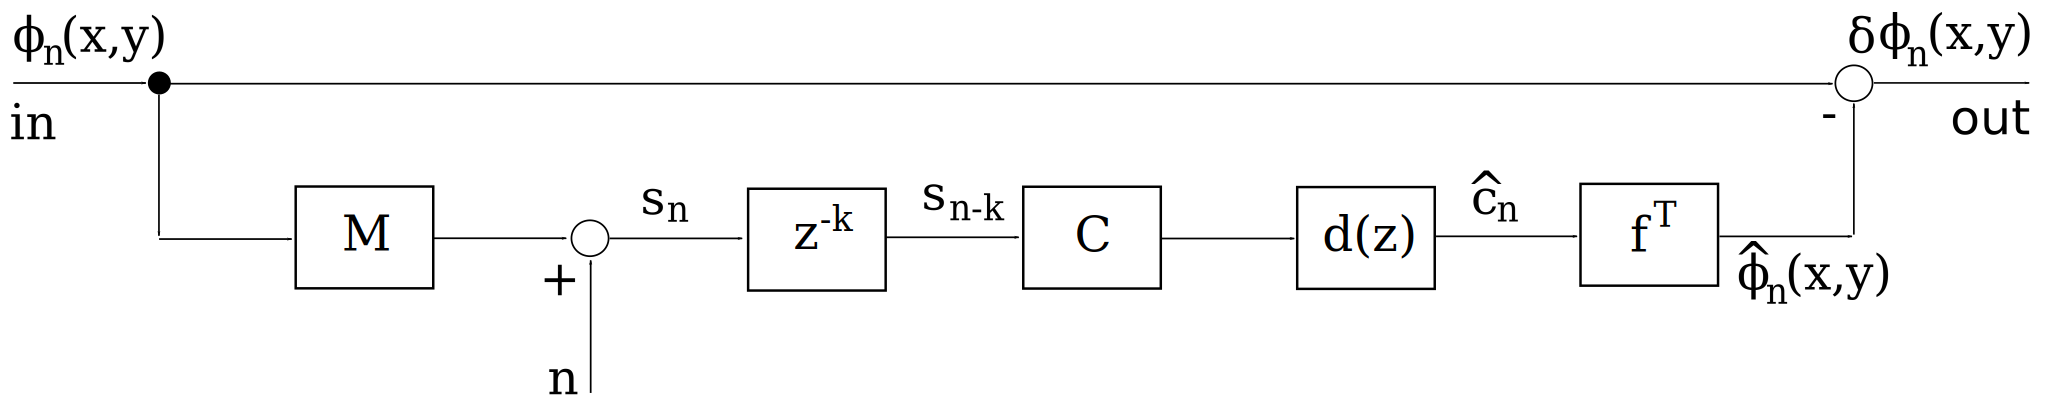
\includegraphics[width = 0.9\textwidth]{Forward.png} \\
 (a) \\
 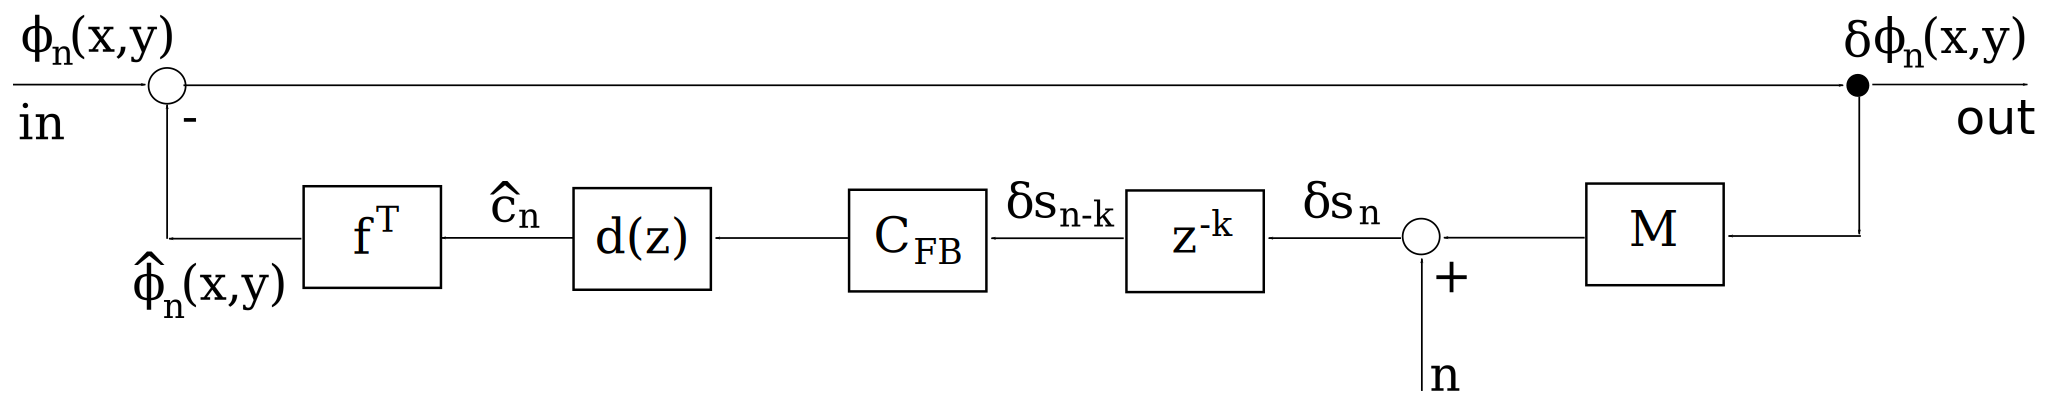
\includegraphics[width = 0.9\textwidth]{Back.png} \\
 (b) \\
\end{tabular}
\end{center}
\caption{Open-loop (a) and closed-loop (b) AO controller block diagrams.}
\label{fig:forward-back}
\end{figure}

Simplified signal block diagrams for an AO system in open-loop and closed-loop
configurations are shown on Fig. \ref{fig:forward-back}.
The system dynamics are modeled by adding: 1)
$k$-step signal delay element with $z$-domain transfer function $z^{-k}$ to
account for delays in sensor and controller; 2) a filter with $z$-domain
transfer function (matrix) $d(z)$ to account for the DM dynamic
effects. It is possible to derive a relationship between the open-loop (or
\emph{feedforward})
reconstructor $\mathcal{R}$ and the closed-loop (or \emph{feedback}) one
$\mathcal{R}_{FB}$ by noticing that, to deliver the same output signal, it
should be
\begin{equation} \label{eq:open-to-close}
  \mathcal{R} \bm{s} = \mathcal{R}_{FB} \delta \bm{s}.
\end{equation}
From the diagrams:
\begin{equation} \label{eq:sopen-to-sclose}
	\delta \bm{s}(z) = \bm{s}(z) - z^{-k} d(z) \mathcal{M} ( \bm{f}^{T}
	\mathcal{R}_{FB} \delta \bm{s}(z) )
\end{equation}
$$
  = \bm{s}(z) - z^{-k} d(z) \mathcal{DR}_{FB} \delta \bm{s}(z),
$$
where $\mathcal{D} = \mathcal{M} (\bm{f}^{T})$ is the \emph{poke matrix}
\index{poke matrix}
relating action of each DM influence function on the WFS measurements.
Substitution of Eq. (\ref{eq:sopen-to-sclose}) into Eq.
(\ref{eq:open-to-close}) yields
\begin{equation} \label{eq:fw-to-fb}
	\mathcal{R}_{FB} = \mathcal{R}
	( \mathcal{I} - z^{-1} d(z) \mathcal{RD} )^{-1}.
\end{equation}

The transfers from input wavefront phase $\phi(n)$ to the AO system
residual phase error $\delta \phi(n)$ (\emph{error rejection transfer
function}): \index{error rejection transfer function} for the feedforward and
feedback controllers shown on Fig. \ref{fig:forward-back} are:
\begin{equation} \label{eq:forward-transfer}
	(\phi \rightarrow \delta \phi)(z) =
	\mathcal{I} -
	z^{-k} d(z) \mathcal{D} \mathcal{R};
\end{equation}
\begin{equation} \label{eq:feedback-transfer}
	(\phi \rightarrow \delta \phi)_{FB}(z) =
	( \mathcal{I}+z^{-k} d(z) \mathcal{D} \mathcal{R}_{FB} )^{-1}.
\end{equation}

The open-loop reconstructor $\mathcal{R}$ can also
be used directly in the \emph{pseudo open-loop} \index{pseudo
open-loop} (POL) setting of the closed-loop control when the open-loop
measurement is approximately restored
through an internal model for the DM. In the case of linear internal model the
approximate (pseudo) open-loop WFS measurement $\hat{\bm{s}}$ is
\begin{equation} \label{eq:wfs-restoration}
	\hat{\bm{s}} = \delta \bm{s} + \mathcal{D} \bm{c}.
\end{equation}
Block diagram for a dynamic MMSE controller working in the POL regime is
shown on Fig. \ref{fig:POL}. The integrator/corrector filter $g(z)$ is used to
produce the absolute DM
commands from differential ones in a way ensuring system stability and dynamic
error minimization.
\begin{figure}[htp]
\begin{center}
 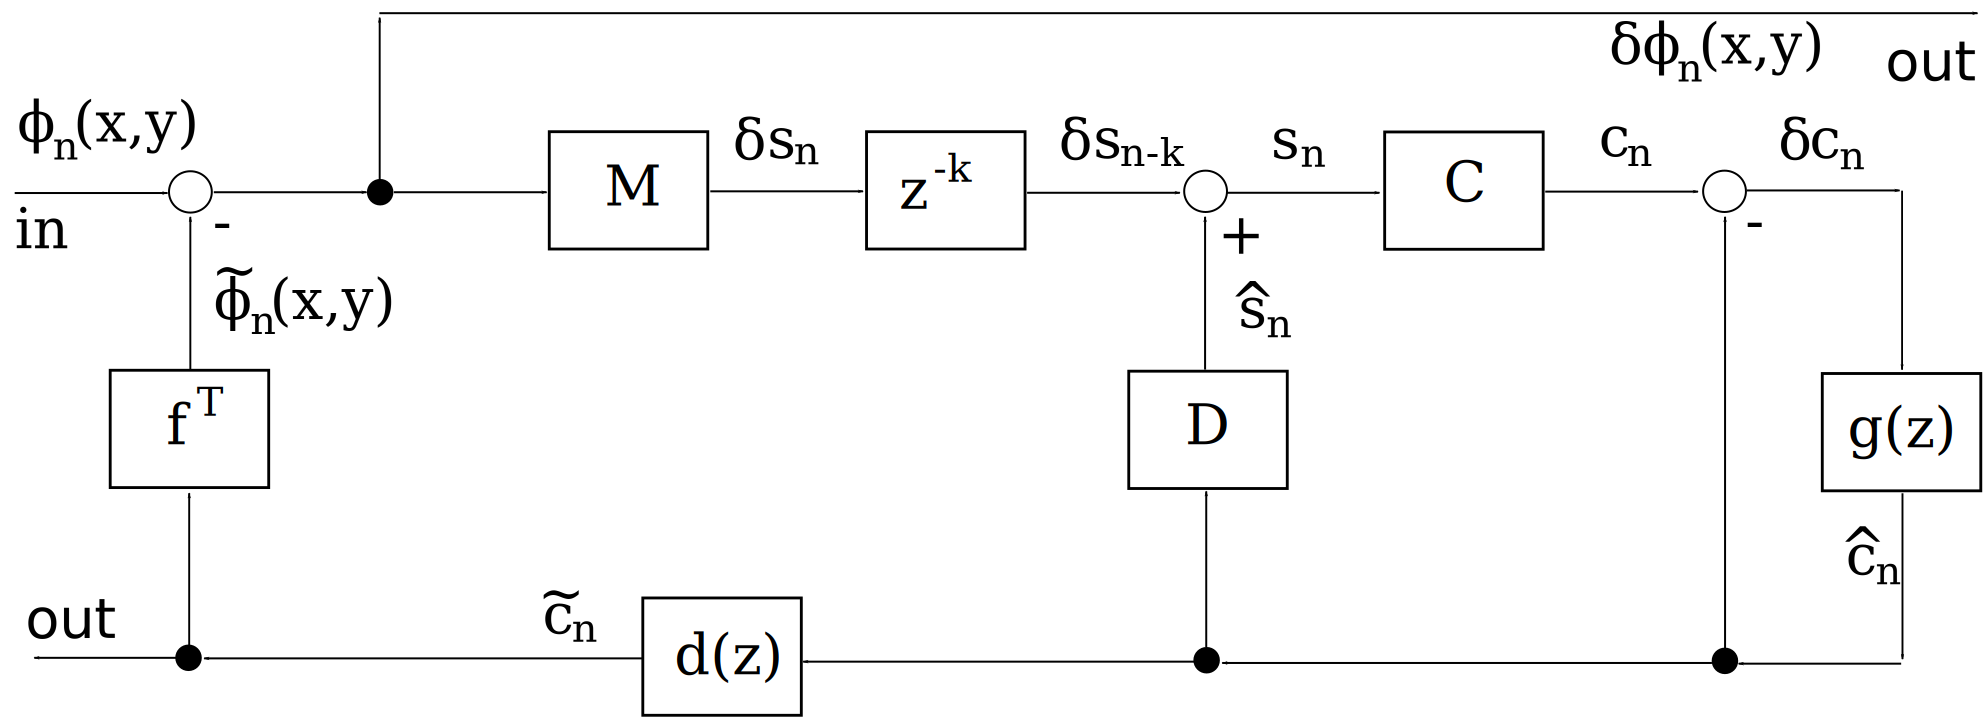
\includegraphics[width = 0.8\textwidth]{POL.png}
\end{center}
\caption{Pseudo Open-Loop MMSE controller block diagram.}
\label{fig:POL}
\end{figure}

The set of dynamic equations for the POL controller is:
\begin{align}
  \texttt{(pseudo open-loop measurement)} \nonumber \\
	\bm{s}(n) = \delta \bm{s}(n-k) + \hat{\bm{s}}(n); \label{eq:POL-meas} \\
	\texttt{(pseudo open-loop command)} \nonumber \\
  \bm{c}(n) = \mathcal{R} \bm{s}(n); \label{eq:POL-est} \\
  \texttt{(command increment)} \nonumber \\
  \delta \bm{c} = \bm{c}(n) - \hat{\bm{c}}(n); \\
  \texttt{(integrator/corrector state space equations, see Appendix
  \ref{app:DF})} \nonumber \\
  \bm{x}^{g}(i+1) = \mathcal{A}^{g} \bm{x}^{g}(n) +
                    \mathcal{B}^{g} \delta \bm{c}(n), \\
  \hat{\bm{c}}(n) = \mathcal{C}^{g} \bm{x}^{g}(n) +
                    \mathcal{D}^{g} \delta \bm{c}(n); \\
  \texttt{(pseudo open-loop measurement estimate)} \nonumber \\
  \hat{\bm{s}}(n) = \mathcal{D} \hat{\bm{c}}(n).
\end{align}
Two important transfer functions (matrices) can be derived from the Fig.
\ref{fig:POL} diagram: 1) the transfer from WFS output $\delta \bm{s}(n)$ to
controller output $\hat{\bm{c}}(n)$ (\emph{controller transfer function}):
\index{controller transfer function}
\begin{equation} \label{eq:WFS-to-Control}
	(\delta \bm{s} \rightarrow \hat{\bm{c}})_{POL}(z) =
	z^{-2} g(z) \left[ \mathcal{I} +
	g(z) (\mathcal{I}-\mathcal{RD}) \right]^{-1} \mathcal{R},
\end{equation}
and 2) the error rejection transfer function:
\begin{equation} \label{eq:phase-to-error}
	(\phi \rightarrow \delta \phi)_{POL}(z) =
	\left[ \mathcal{I} + d(z) \bm{f}^{T}
	(\delta \bm{s} \rightarrow \hat{\bm{c}})_{POL}(z) \mathcal{D} \right]^{-1}.
\end{equation}

Being formally equivalent, feedforward, feedback and POL controllers have
different stability and error propagation properties.

\subsection{Tomographic MMSE reconstructor}
\label{subsec:MMSE-tomo}

\mbox{}

A generalization of the single-conjugate AO control is the \emph{star-oriented
tomography}. \index{star-oriented tomography}

%We also use the assumption that the sensor noise is not correlated with the
%atmospheric turbulence, i.e.
%\begin{equation} \label{eq:turb-cross-noise}
	%\langle \bm{n} \bm{x}^{T} \rangle = 0,
%\end{equation}
%$$ \langle \bm{n} \bm{x}_{Sc}^{T} \rangle = 0. $$

%Fig. \ref{fig:POL} diagram and the equations thereafter make the main building
%block for the dynamic AO control algorithms. We will call it the
%\emph{standard AO control}. \index{standard AO control}
%The five \emph{system matrices}: \index{system matrices}
%$\langle \bm{x}_{Sc} \bm{x}^{T} \rangle$,
%$\langle \bm{x}_{Sc} \bm{x}^{T} \rangle$, $\langle \bm{n}_{s} \bm{n}_{s}^{T}
%\rangle$, $\mathcal{D}$, $\mathcal{F}$, describe interaction between the parts
%of an AO system and the $z^{-k}$, $g(z)$, $d(z)$ \emph{system filters}
%\index{system filters} describe the system dynamics
%in first approximation. These data are the AO system model inputs.
%In order to describe these inputs in more detail one has to elaborate into
%the GMT LTAO system structure.

\subsection{GMT LTAO sub-systems}
\label{subsec:ltao-sub-systems}

\mbox{}

According to the \emph{split control concept} \index{split control concept}
the entire GMT LTAO system can be viewed as a set of weakly interacting
control sub-systems (feedback loops, see Fig. TBD):
\begin{enumerate}
	\item The \emph{ASM high order LGS-based} (ASM HO LGS) \index{ASM high order
	LGS-based control loop}
	control loop intended to reject high spatial order atmospheric/telescope
	aberrations and using the LGS return for WFS measurements. This channel has
	the following features:
	\begin{itemize}
		\item This channel works in closed-loop behind ASM.
		\item Target is $\phi_{Sc}$ is the wavefront from a scientific object.
		\item Reference is $\phi_{LGS}$ is the wavefront from 6 LGSs.
	  \item The control commands generated in this channel are sent to the ASM.
	  \item The wavefront sensors for this channel are the 6 LGS WFSs.
	  \item The sampling rate is the one of the LGS WFSs.
	\end{itemize}

	\item The \emph{ASM low order NGS-based} (ASM LO NGS) or ``truth'' control
	loop is used to provide low order ASM correction, which is impossible to
	determine from the LGSs. Another possible use of the LO NGS WFS is to sense
	the primary segment differential pistons. \index{ASM low order NGS-based
	control loop} This channel has the following features:
	\begin{itemize}
		\item This channel works in closed-loop behind ASM and OI DM.
		\item Target is the wavefront $\phi_{Sc}$ from a scientific object.
		\item Reference is the wavefront $\phi_{NGS}$ from one NGS.
	  \item The control commands generated by this channel are sent to ASM.
	  \item The wavefront sensor for this channel is the LO NGS WFS (``truth
	  sensor'').
		\item The sampling rate is the one of the LO NGS WFS.
	\end{itemize}

	\item The \emph{ASM tip/tilt NGS-based} (ASM TT NGS) \index{ASM tip/tilt
	NGS-based control loop} control loop
	intended to sense and correct the waveront tip/tilt in the scientific object
	direction using a natural guide star. This channel has
	the following features:
	\begin{itemize}
		\item This channel works in closed-loop behind ASM and OI DM.
		\item Target is the wavefront $\phi_{Sc}$ from a scientific object.
		\item Reference is the wavefront $\phi_{NGS}$ from one NGS.
		\item The control commands generated in this channel are sent to the ASM.
		\item The wavefront sensor for this channel is a quad-cell tip/tilt NGS
		(TT NGS) WFS.
	  \item The sampling rate is the one of the TT WFS.
	\end{itemize}

  \item The \emph{OI DM high order LGS-based} (OI DM HO LGS)
  \index{OI DM high order LGS-based control loop} control loop is for
  correcting the NGS wavefront by the OI DM in order to improve performance of
  the NGS TT channel. This channel has the following features:
  \begin{itemize}
	  \item This channel works in closed-loop behind ASM.
	  \item Target is the wavefront $\phi_{NGS}$ from a NGS.
	  \item Reference is the wavefront $\phi_{LGS}$ from 6 LGSs.
	  \item The control commands generated in this channel are sent to OI DM.
	  \item The wavefront sensors for this channel are the 6 LGS WFSs.
    \item The control algorithm is closed-loop with respect to the ASM but
    open-loop with respect to OI DM.
	  \item The sampling rate is the one of the LGS WFSs.
	\end{itemize}

	\item The \emph{OI DM low order NGS-based} (OI DM LO NGS) control loop is
	to provide the low order OI DM correction, which is not possible to
	determine from the LGSs.  \index{OI DM low order NGS-based control loop}
	This channel has the following features:
	\begin{itemize}
		\item This channel works in closed-loop behind ASM and OI DM.
		\item Target is the wavefront $\phi_{NGS}$ from a NGS.
		\item Reference is the wavefront $\phi_{NGS}$ from the same NGS.
		\item The control commands generated by this channel are sent to OI DM.
	  \item The wavefront sensor for this channel is the LO NGS WFS.
		\item The sampling rate is the one of the LO NGS WFS.
	\end{itemize}

\end{enumerate}

One has also to mention some auxiliary control channels used for or together
with LTAO. They are not based on the standard AO control and use other control
approaches.
\begin{enumerate}
	\item \emph{LGS focus stabilization subsystem} \index{LGS focus stabilization
	subsystem} is used for adjusting the LGS WFS
	module focal plane to follow slow LGS position changes in the sky. This
	channel has the following features:
	\begin{itemize}
		\item The feedback signal is the global focus mode extracted from the 6
		LGS WFS measurements.
		\item The control is applied to a servo actuator moving the whole LGS WFS
		module to adjust to the focus. The controller needs to be optimized to the
		(actuator + LGS module) dynamics.
	\end{itemize}
	\item \emph{LGS pupil de-rotation subsystem} \index{LGS pupil de-rotation
	subsystem} is used for compensation of the exit
	pupil rotation on the LGS module induced by changes in the telescope pointing.
	This channel has the following features:
	\begin{itemize}
		\item The feedback signal for this channel is the correlated part of the
		LGS WFS spot motions.
		\item The control is applied to a servo actuator rotating the whole LGS
		WFS module to adjust to the pupil rotation.
	\end{itemize}
	\item \emph{OI WFS acquisition/image stabilization subsystem} \index{OI WFS
	acquisition/image stabilization subsystem} is used find the NGS
	in the telescope field-of-view, to point the light from an NGS to the
	OI WFS detectors and stabilize it. This channel has the following features:
	\begin{itemize}
		\item An acquisition camera is used to provide a signal to the controller.
		\item The control is applied to a two degree-of-freedom actuator attached
		to the acquisition flat mirror located inside OI WFS module.
		\item The acquisition camera and mirror work in closed-loop regime behind
		ASM and OI DM.
	\end{itemize}
	\item \emph{GMT phasing subsystem} \index{GMT phasing subsystem} is an
	\emph{active optics} system that keeps the telescope aligned, phased and
	shape-stabilized.
\end{enumerate}
The auxiliary control sub-systems do not directly participate in the AO
correction but the errors in these systems become the additional error inputs
for the main AO controllers thus upsetting indirectly the AO system
performance.

%!!!!!!
%Let the low order wavefront part to be removed from the wavefront $\bm{x}_{Sc}$
%by the $\mathcal{P}_{HO}$-matrix or extracted from $\bm{x}_{Sc}$ by the
%$\mathcal{P}_{LO}$-matrix can be presented as a linear combination
%$$
  %\bm{x}_{LO} = \sum_{i=1}^{L} w_{i} \bm{q}_{i}
%$$
%of the mutually orthonormal modes $\{ \bm{q}_{i} \}_{i=1}^{L}$, then the
%projection matrices are:
%\begin{eqnarray} \label{eq:l0-ho-projectors}
	%\mathcal{P}_{LO} &=& \mathcal{QQ}^{T}, \\
	%\mathcal{P}_{HO} &=& \mathcal{I} - \mathcal{QQ}^{T}, \\
	%\mathcal{Q} &=& [\bm{q}_{1} \, ... \, \bm{q}_{L}], \,\,
	%\mathcal{Q}^{T} \mathcal{Q} = \mathcal{I}.
%\end{eqnarray}
%In case $\{ \bm{q}_{i} \}_{i=1}^{L}$ are not orthonormal but linearly
%independent, they can be easily orthonormalized by means of the
%QR-decomposition.
%!!!!!! \\

\subsubsection{ASM HO LGS controller algorithm}
\subsubsection{ASM LO NGS controller algorithm}
\subsubsection{ASM TT NGS controller algorithm}
\subsubsection{OI DM HO LGS controller algorithm}
\subsubsection{OI DM LO NGS controller algorithm}

%The OI DM HO LGS controller is a modification of the standard AO algorithm
%with the following changes:
%\begin{enumerate}
	%\item The OI DM HO LGS estimator matrix $\mathcal{E}_{HO,OIDM}$ is computed
	%by Eq. (\ref{eq:estimator}), where the wavefront $\bm{x}_{Sc}$ from a science
	%target is replaced with wavefront $\bm{x}_{NGS}$ from the NGS:
	%\begin{equation} \label{eq:OI-DM-H)-LGS-estimator}
	  %^{ngs}\mathcal{E}_{ho}^{lgs} = ^{NGS}\mathcal{P}_{HO}
	%\end{equation}
	%\item The POL measurement equation (\ref{eq:POL-meas}) is replaced with
	%\begin{equation} \label{eq:POL-OIDM}
		%\bm{s}(n) = \delta \bm{s}(n) + \hat{\bm{s}}_{ASM}(n),
	%\end{equation}
	%where $\delta \bm{s}(n)$ is the LGS WFS closed-loop measurement, same as
	%that for HO ADM LGS controller input,
	%$\hat{\bm{s}}_{ASM}(n)$ is an estimate of LGS WFS measurement due to
	%commands sent to ASM by the HO ASM LGS, LO ASM NGS and TT ASM NGS
	%controllers.
	%\item There is no integrator in the HO OI DM control loop because the LGS
	%WFSs are not behind OI DM. Thus
	%\begin{equation} \label{eq:H)-OIDM-commands}
		%\hat{\bm{c}}_{HO,OIDM} (n) = \mathcal{E}_{HO,OIDM} \bm{s}(n)
	%\end{equation}
	%is the HO open-loop OI DM control command.
	%\item Since OI DM is behind the ASM, the differential command $\delta
	%\hat{\bm{c}}_{OIDM}$ to be sent to OI DM should take into account the ASM
	%correction:
	%\begin{equation} \label{eq:OIDM-balance}
		%\delta \hat{\bm{c}}_{OIDM} = \hat{\bm{c}}_{OIDM} -
		%\hat{\bm{c}}^{ASM}_{OIDM},
	%\end{equation}
	%where $\hat{\bm{c}}^{ASM}_{OIDM}$ is the best fit of the ASM correction
	%wavefront by the OIDM:
	%\begin{equation} \label{eq:ASM-to-OIDM-fit}
		%\hat{\bm{c}}^{ASM}_{OIDM} = \arg \min_{\forall \bm{c}}
		%|\mathcal{F} \hat{\bm{c}}_{ASM} - \mathcal{F}|^{2}
	%\end{equation}
%\end{enumerate}

\subsection{GMT LTAO system fusion}
\label{subsec:ltao-system-fusion}

TBD

\subsection{GMT LTAO system dynamic analysis}
\label{subsec:ltao-dynamics}

TBD

\subsection{GMT LTAO system error and robustness analysis}
\label{subsec:ltao-errors}

TBD